\chapter{A estratégia de produção} 
\label{chap:estrategia_da_producao} 
Neste capítulo será explicado como formular a estratégia de produção de uma empresa industrial visando atender o seu objetivo geral de desempenho. Uma estratégia de produção consiste em converter as intenções contidas em ações práticas como projetos concretos, planos e melhorias. Para isso, será explicado como a função de produção tem importância estratégica para a organização industrial e como definir o conteúdo que estará presente na estratégia visando atender o objetivo geral de desempenho escolhido. 

Por fim, a seção \ref{sec:estrategia_da_producao_aplicacao} mostrará como foi elaborado a estratégia de produção da empresa \textit{SunBurn}. 

\section{Sec1} 
\label{sec:estrategia_da_producao_sec1} 
A estratégia de operações analisa o processo global da função de produção da empresa industrial como um todo. Por isso, ela preocupa-se, se existir, com as outras partes da corporação, com as outras partes da unidade de negócio (marketing, finanças, recursos humanos entre outras) e com o local onde o negocio esta inserido (concorrentes, clientes externos etc). Além disso, tem o objetivo de manter a área de operações adaptadas às mudanças desses fatores ambientais, portanto, a operação enfrentará melhor os problemas futuros. Com isso, é garantido que as organizações possa ter níveis sustentáveis de vantagens competitivas \cite{correa2000administracao}.

Ainda segundo o autor, a matriz \textit{importância x desempenho}, conforme mostra a Figura \ref{fig:matriz_importancia_desempenho},  é uma ferramenta que deve ser utilizada para a priorização dos objetivos da função de operações. Essa matriz, possui duas dimensões: uma delas refere-se à importância relativa dada pelos clientes aos critérios de desempenho, utilizando a escala de nove pontos e a outra envolve uma classificação, também com uma escala de nove pontos, do desempenho de cada objetivo contra os níveis de desempenho atingidos pelos concorrentes.

\begin{figure}[H]
  \caption{Matriz importância x desempenho}
  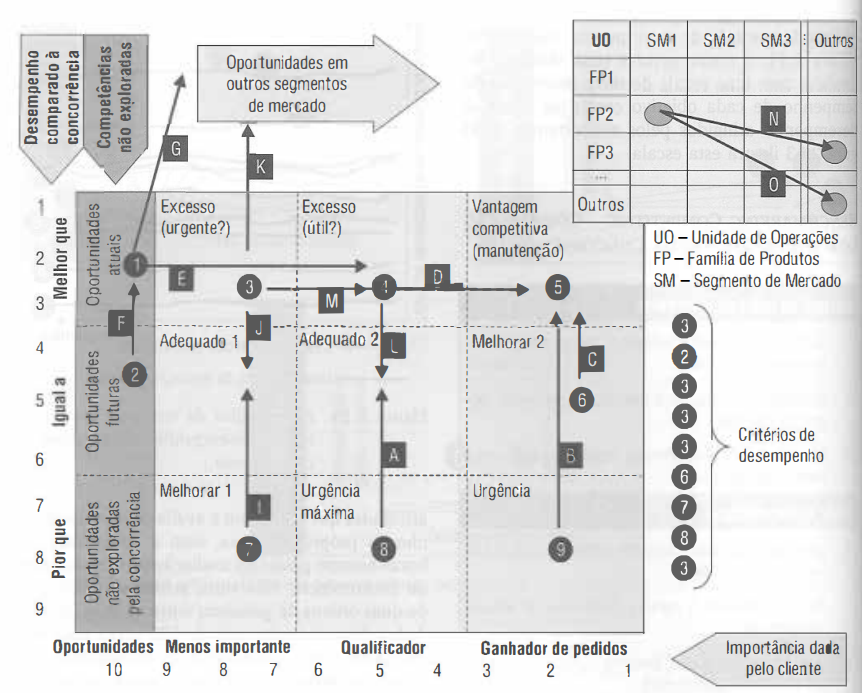
\includegraphics[width =1\textwidth]{images/impor_desem.png}
  \label{fig:matriz_importancia_desempenho}
  \caption*{Fonte: \cite{correa2000administracao}}
\end{figure}

O cruzamento das duas dimensões (importância dos critérios para o mercado e desempenho nos critérios comparado à concorrência) permite identificar regiões específicas na matriz, conforme mostrado na figura acima.




\section{Aplicação Prática} 
\label{sec:estrategia_da_producao_aplicacao}